\documentclass[UTF8]{ctexart}
\usepackage{dirtree}
\usepackage{listings}
\usepackage{xcolor}
\usepackage{graphicx}
\usepackage{enumerate}
\usepackage[a4paper]{geometry}
\usepackage{amsmath,amsthm,mathtools,amsfonts,amssymb}
\usepackage{diagbox}
\usepackage{multirow,makecell}
\usepackage{float}
\usepackage{url}
\usepackage[nottoc]{tocbibind}
\usepackage[colorlinks=true, linkcolor=black]{hyperref}
\usepackage{float}
\newcommand{\reff}[1]{图\ref{#1}\ }
\newcommand{\refd}[1]{\emph{定义}.\ref{#1}\ }
\newcommand{\refe}[1]{\emph{公式}.\ref{#1}\ }
\newcommand{\reft}[1]{\emph{定理} \ref{#1}\ }
\newcommand{\refl}[1]{\emph{引理} \ref{#1}\ }
\newcommand{\refp}[1]{\emph{推论} \ref{#1}\ }
\newtheorem*{bz}{倍增算法}
\newtheorem{define}{定义}
\newtheorem{theory}{定理}
\newtheorem{lemma}{引理}
\newtheorem{derive}{推论}

\geometry{bottom=2cm,left=1cm,right=1cm}
%插入代码样式设置
\lstset{
 columns=fixed,
 numbers=left,                                        % 在左侧显示行号
 numberstyle=\tiny\color{gray},                       % 设定行号格式
 basicstyle=\small\ttfamily,
 frame=none,                                          % 不显示背景边框
 backgroundcolor=\color[RGB]{245,245,244},            % 设定背景颜色
 keywordstyle=\color[RGB]{40,40,255},                 % 设定关键字颜色
 numberstyle=\footnotesize\color{darkgray},           
 commentstyle=\color{gray}\ttfamily,                  % 设置代码注释的格式
 stringstyle=\rmfamily\slshape\color[RGB]{128,0,0},   % 设置字符串格式
 showstringspaces=false,
 breaklines=true,
 language=c++
}
\title{大作业}
\author{张配天-2018202180}

\begin{document}
    \maketitle
    \tableofcontents
    \clearpage
    \section{匹配结果}
    \begin{table}[H]
        \centering
        \begin{tabular}{c|c|c|c}
            \hline
            &短串1&短串2&短串3\\
            \hline
            在10亿长度字符串(助教给的1G)中的匹配结果&没有匹配&从\textbf{423989716}开始&从\textbf{0}开始\\
            \hline
        \end{tabular}
    \end{table}
    \section{功能说明}
    \subsection{实现功能}
    用$O(m)$时间复杂度找出一个长度为$m$的短字符串在一个长度为$n$的长字符串中的精确匹配,$n>>m$。
    \subsection{算法运行时间}
    \begin{table}[H]
        \centering
        \begin{tabular}{cccc}
            \hline
            数据规模&构建\emph{Burrows-Wheeler Matrix}用时&查询长度为10000的字符串用时&查询长度为200000的字符串用时\\
            20万&平均0.2s&0s&0s\\
            100万&平均1s&0s&0s\\
            1亿&平均280s&0s&0s\\
            10亿&平均4400s&0s&0s\\
            \hline
        \end{tabular}
    \end{table}
    \section{输入输出}
    \subsection{输入}
    \begin{itemize}
        \item \textbf{长串文件路径(一行);}
        \item \textbf{短串文件路径(一行);}
    \end{itemize}
    
    \begin{figure}[H]
        \label{fig1}
        \centering
        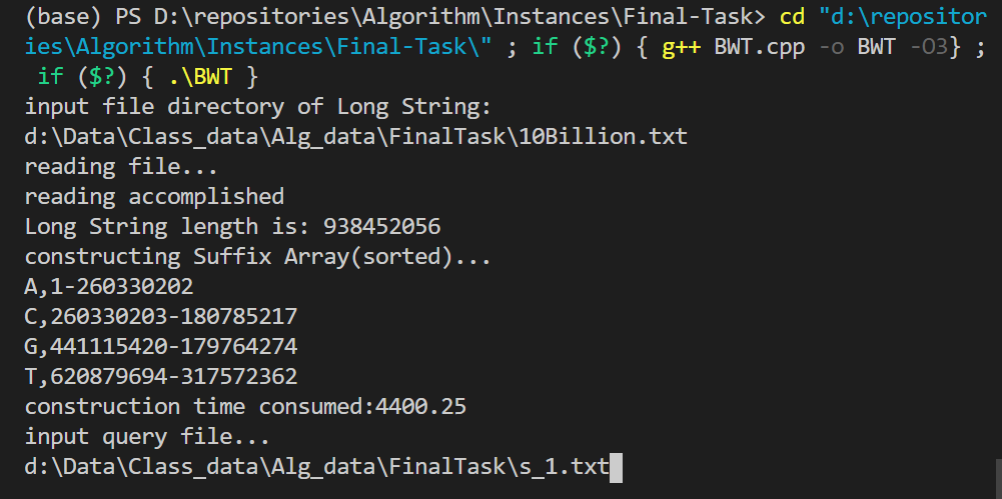
\includegraphics[width=12cm]{../Resources/ft_input.png}
        \caption{输入}
    \end{figure}
    \subsection{输出}
    \begin{itemize}
        \item 输入长串txt文件后程序将自动读入长串并输出长度, 如\reff{fig1}所示;之后程序
        开始构建\emph{Burrows-Wheeler Matrix}, 并在候检结束后输出\textbf{构建时间和长串的单词表(ATCG各有多少个, 以及开始的位置)}。
        \item 手动输入要查询的短串的文件路径, 程序会输出\textbf{匹配结果的个数}, 并将\textbf{每一个结果在长串中的开始位置及匹配字符串输出到results.txt文件中};如果没有匹配, 则会输出\textbf{NO MATCHING!}
    \end{itemize}
    \begin{figure}[H]
        \centering
        \label{fig2}
        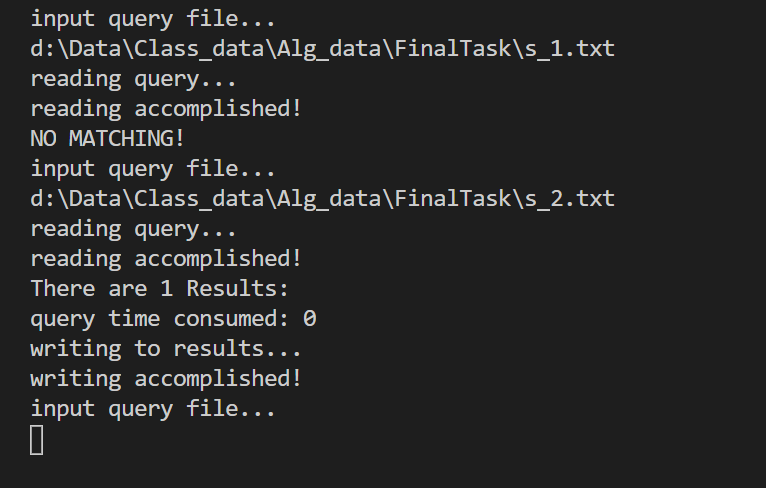
\includegraphics[width=12cm]{resources/ft_output.png}
        \caption{查询}
    \end{figure}

    \section{设计原理说明}
    \subsection{后缀排序}
    \subsubsection{输入}
    字符串$\mathcal{S}, |\mathcal{S}| = N$%。$\mathbb{M}$, 即字符串$S$的\emph{rotation}构成的矩阵。
    \subsubsection{输出}
    字符串$\mathcal{S}', |\mathcal{S}'| = N+1$的后缀数组$V$ (按照字母表顺序排好序)%$\mathbb{M}^s$, 即按照字母前后顺序排好序的$\mathbb{M}$。
    \subsubsection{算法思路}
    \noindent \textbf{核心: }给$\mathcal{S}$最后加一个结束符$@$形成$\mathcal{S}'$, 默认该结束符小于任何一个字母;
    在此基础上构建$\mathcal{S}'$的BWM(\emph{Burrows-Wheeler Matrix} / \emph{rotation matrix}) $\mathbb{M}$ 有$N+1$行$N+1$列;

    \begin{define}
        \label{def1}
        对于长为$N$的字符串$\mathcal{S} = [s_1,...,s_N]$, 其后缀(\textbf{suffix})定义为$\mathcal{S}[i:N+1]$即从第$i$个字符开始到最后一个字符的$\mathcal{S}$的子串;
        令$A=[1,...,n]$代表$\mathcal{S}$的全部后缀的开始位置, 则后缀数组(\textbf{suffix array})$V$定义为按照字母表顺序排好序后每一个后缀对应的开始位置, 满足\begin{equation}
            S[V[i]:N+1] < S[V[i+1]:N+1]
        \end{equation}
    \end{define}

    \begin{theory}
        \label{the1}
        对$\mathbb{M}$进行排序, 等价于对$\mathbb{M}$的中每一行到$@$为止的字符串(即$\mathcal{S}$的每一个suffix)进行排序。
    \end{theory}
    \begin{proof}
        由于$\mathbb{M}$中每一行都是上一行向右偏移一位字符形成的, 且每一行只有一个$@$, 因此在矩阵$\mathbb{M}$中每一
    列仅有一个$@$;对于$\mathbb{M}$中的任意两行$r_i$和$r_j$, 不妨设$r_i[u] = @, r_j[v] = @$且$u<v$, 那么有\begin{enumerate}
        \item $r_i[:u] < r_j[:u]$, 则$r_i < r_j$;
        \item $r_i[:u] == r_j[:u]$, 则$r_i < r_j$因为$r_i[u] = @ < r_j[u]$一定成立
        \item $r_i[:u] > r_j[:u]$, 则$r_i> r_j$;
    \end{enumerate}
    \end{proof}
    
    \textbf{因此, 根据\refd{def1} 给\emph{BWM}排序就转化成了给$\mathcal{S}'$的所有后缀进行排序的问题。}
    \par 尽管将\emph{BWM}转化为后缀数组, 将$N*N$的规模转化为$(N+1)*(N+1)/2$, 但本质上没有显著降低复杂度, 还是要对
    给N个后缀字符串排序的时间复杂度仍为$O(N*N*lgN)$, 
    当字符串很长(\emph{比如1亿的长串})时, 效率很低下。

    因此这里提出使用\textbf{“倍增算法”}进行排序。此算法利用了后缀字符串均为原字符串的子串的性质;
    
    \begin{bz}  记从$i$位置开始到$j$位置结束的后缀字符串$\mathcal{S'}[i:j]$为$s_{i,j}$, 那么对$s_{i,N}$排序相当于先对$s_{i,2i}$排序, 再对$s_{2i,3i}$排序。
    而对$s_{2i,3i}$的排序包含在对$s_{i,2i}$的排序结果中(因为由\reft{the1}, $s_{2i,3i}$作为$\mathcal{S'}$的\emph{cyclic rotation} 也参与了
    对$s_{i,2i}$的排序), 即可以在我们排序$s_{i,2i}$的时候同时得到, 因此可以节省计算步骤, 将$O(N)$级别的循环降为$O(lgN)$级别的循环。
    \end{bz}

    \par\noindent 具体来说, 记待排序后缀字符串形成的矩阵为$M$, 有\textbf{倍增排序}算法步骤如下:
    \begin{enumerate}[I.]
        \item 对$M$中每一行赋两个初始评分, \begin{align}
                    M[i].rank[0]&=ascii_{M[i][0]} - ascii_{@}\\
                    M[i].rank[1]&=ascii_{M[i][1]} - ascii_{@}
            \end{align}
        则此时$rank_1$反映了前两个字符之间的大小关系;
        \item 依照$rank_1,rank_2$对$M$进行排序, 注意如果$rank_2^i = rank_2^j$时才需要比较$rank_1$, 否则直接根据$rank_2$得到相对顺序;排序完成后
        $M$中的各个字符串已经按照前两个字母的相对顺序排好;
        \item 初始化$k=2$;
        \item %如果第$i$行的后缀数组的$rank_1$和第$i-1$行的后缀数组的$rank_1$相等, 则$$
              更新每一行的第一个评分, 初始化$rank=0$,\begin{equation}
                M[i].rank[0] = \begin{cases}
                    rank &M[i].rank == M[i-1].rank\\
                    ++rank &M[i].rank \neq M[i-1].rank
                \end{cases}
              \end{equation}

              则此时$M$中每一行$M[i].rank[0]$概括了字符串前$k$位字母的相对顺序;
        \item 更新每一行的第二个评分, \begin{equation}
            M[i].rank[1] = M[j].rank
        \end{equation}
        其中\begin{equation}
            M[j] = M[i][k:N+1]
        \end{equation}
        则此时$M$中的每一行$M[i].rank[1]$概括了字符串$k\thicksim 2k$位字母的相对顺序, 而这个相对顺序\textbf{并不是通过排序得到的, 而是直接查表获得(在第4步保存$V[j]$对应的$M[i]$, 则第五步可以通过查找$V[j+2]$对应的$M[i']$直接得到)}。
        \item 更新$k = k*2$, 如果$k < N+1$, 那么继续返回第四步。
    \end{enumerate}
    \subsubsection{复杂度分析}
    \begin{theory}
        倍增算法排序的时间复杂度为$O(NlgNlgN)$, 空间复杂度$O(lgN)$
    \end{theory}
    \begin{proof}
        根据上述算法,
        \begin{itemize}
            \item 第一第二步遍历$M$的每一行, 初始化$rank[0],rank[1]$, 复杂度为$O(N)$, 给$N+1$数排序复杂度为$O(NlgN)$, 总复杂度$O(NlgN)$;
            \item 第四步遍历$M$的每一行,更新$rank$, 复杂度为$O(N+1)$;
            \item 第五步给$N+1$个数排序, 复杂度为$O(NlgN)$;
            \item 第六步会重复第四,第五步$O(lgN)$次, 因此总时间复杂度$O(NlgNlgN)$;
        \end{itemize}
        由于使用快速排序, 是原址排序, 且排序对象\textbf{并非字符串, 而是两个rank值, 只占用$O(1)$的空间, 递归调用$lgNlgN$次, 但每一次调用的额外空间都可以重复使用, }因此总空间复杂度为$O(lgN)$。
    \end{proof}
    % \begin{align}
    %     2^0 + 2^1 + \cdots + 2^k &= N+1\\
    %     \implies 2^{k+1} - 1 &= N+1\\
    %     \implies k = 
    % \end{align}
    \subsection{构建BWM的第一列,最后一列和tally数组}
    \subsubsection{输入}
    $\mathcal{S}'$和后缀数组$V$
    \subsubsection{输出}
    \begin{itemize}
        \item $F$: BWM的第一列;
        \item $L$: BWM的最后一列;
        \item $vocab\_idx$: 长串中的每个字母对应在$tally$数组中的列号;
        \item $vocab\_count$: 长串中的每个字母出现频率;
        \item $tally$: $(N+1) * (M)$的数组, 保存$last$中每一行的各个字母出现次数;
    \end{itemize}
    \subsubsection{算法思路}
    在算出按照字母序排好的后缀数组$V$后, 需要根据$V$生成\emph{BWT}算法需要的第一列和最后一列, 以及\emph{FM}算法需要的tally数组。
    \begin{lemma}
        \label{lem1}
        记$\mathbb{M}$的第一列为$F$, 则
        \begin{equation}
            F[i] = \mathcal{S}'[SA[i]]
        \end{equation}
    \end{lemma}
    \begin{proof}
        $\mathbb{M}$的每一行都是相同的字符串$\mathcal{S}'$的\emph{cyclic rotation}, 因此初始情况下自然有$F[i] = \mathcal{S}'[SA[i]]$, 又因为后续的
        排序不改变$F$中的元素, 只改变其位置, 因此恒有$F[i] = \mathcal{S}'[SA[i]]$, 
    \end{proof}

    \begin{theory}
        记BWM的第一列为$F$, 最后一列为$L$, 那么有\begin{align}
            L[i]& = \mathcal{S'}[V[i] - 1]
        \end{align}
    \end{theory}
    \begin{proof}
        首先, $V[i]$是代表$\mathcal{S}'[i:N+2]$, 且所有$V$已经根据$\mathcal{S}'[i:N+2]$排序, 
        且根据\refl{the1}此排序和直接对$\mathbb{M}$排序得到的顺序一致;且根据
        \refl{lem1}有\begin{equation*}
            F[i] = \mathcal{S}'[V[i]]
        \end{equation*}
        而$\mathbb{M}$的第一列$F$始终是最后一列$L$的前一个字母, 因此\begin{equation}
            L[i] = \mathcal{S'}[V[i] - 1]
        \end{equation}
        
    \end{proof}
    \noindent 由此, 我们可以仅遍历一次$V$, 并\begin{enumerate}
        \item 计算出$F,L$;
        \item 计算出$\mathcal{S}'$中每个字母出现的次数, 并据此构建$vocab\_idx,vocab\_count$;
        \item 计算出$tally$数组, 即$tally[i][j] = c_i^j$, 代表$vocab\_idx$中第$j$个字母到$F[i]$为止出现的总次数;
    \end{enumerate}
    \subsubsection{压缩存储}
    为了避免tally数组庞大的内存占用, 采用\textbf{检查点(checkpoint)}的方式保存;即不保存整个数组, 而是每隔$\Delta$行, 保存一个\textbf{checkpoint, 即到当前为止L中各字母出现的数量。}

    \subsubsection{复杂度分析}
    由于只需要遍历一遍$V$, 因此有时间复杂度$O(N)$, 假设$\mathcal{S'}$中共有$\Sigma$个不同的字母,则$tally$数组有$\lceil\frac{N+1}{\Delta}\rceil + 1$行$\Sigma$列, 因此有空间复杂度$O(\frac{N\Sigma}{\Delta})$;
    
    \subsection{FM index和查询}
    \subsubsection{输入}
    \begin{itemize}
        \item $F$: BWM的第一列;
        \item $L$: BWM的最后一列;
        \item $V$: 后缀数组;
        \item $q$: 做查询的短串,$|q| = m$;
    \end{itemize}
    \subsubsection{输出}
    \begin{itemize}
        \item 匹配字符串的开始位置;
    \end{itemize}
    \subsubsection{算法思路}
    \begin{theory}
        \label{the2}
        $F$中包含$char$的行之间的相对顺序和$L$中包含$char$的行之间的相对顺序一致
    \end{theory}
    \begin{proof}
        记$F$中包含$char$的行的集合为$\Phi$, 则$\forall \phi_i,\phi_j \in \Phi$, $\phi_i, \phi_j$的相对顺序
        完全由$\phi_i[1:N+2],\phi_j[1:N+2]$决定;同理, 记$L$中包含$char$的行的集合为$\Psi$, 则$\forall \psi_i,\psi_j \in \Psi$, $\psi_i, \psi_j$的相对顺序
        完全由$\psi_i[0:N+1],\psi_j[1:N+1]$决定;\begin{itemize}
            \item 由\reft{def1}, $\mathbb{M}$的每一行和$F,L$都是$\mathcal{S}'$的一个\emph{cyclic rotation}, 
            于是$|\Phi| = |\Psi| = N+1$;
            \item 进一步, $\because \phi_i[1:N+2] = \psi_i[0:N+1] , \phi_j[1:N+2] = \psi_j[0:N+1]$, 所以两者的相对顺序一定一致。
        \end{itemize}    
    \end{proof}
    \begin{define}
        \label{def2}
        \textbf{FM Index}: $L$中的第$k$个$char$在$F$中也对应第$k$个$char$, 并且$F$中的字符串是按照字母表顺序排好的, 因此若$vocab\_idx[char] = r$, 那么
        $char$在$F$中的位置即为\begin{equation}
            \label{e1}
            \sum_{j = 0}^{r-1}vocab\_count[j] + k
        \end{equation}
    \end{define}
    \noindent 根据\textbf{FM Index}, 可以进行query, 步骤如下\begin{enumerate}
        \item \textbf{初始化$k=K$};
        \item \textbf{在$F$中查询$q[k]$, 找到对应的行($\xi= \{i | F[i] = q[k] \wedge rank_1 \leq i \leq rank_2 \}$)};这些行代表$\mathcal{S'}$中以$q[k]...q[K]$为起始字母的后缀字符串;
        \item \textbf{在$L$中查询$q[k-1]$, 找到对应的行($\lambda = \{i | L[i] = q[k-1] \wedge i \in \xi \}$)};这些行代表$\mathcal{S'}$中以$q[k-1]q[k]...q[K]$为起始字符串的后缀字符串;
        \item \textbf{根据$tally, \lambda, vocab\_idx, vocab\_count$和\refe{e1}更新$rank_1, rank_2$};如果$rank_1 > rank_2$则没有查询结果;
        \item \textbf{更新k后重复回到步骤2};如果k=0则查询完毕, 输出$\xi$;
    \end{enumerate}
    \noindent 最后我们就得到了以$q$为起始字符串的后缀字符串在BWM中的行号$\hat{\xi}$, 又根据\refl{lem1}则可以直接得到以$q$为起始字符串的后缀字符串在$\mathcal{S'}$中的位置(即$s_{i,j}$的$i$)。
    \subsubsection{复杂度分析}
    \begin{theory}
        基于\textbf{FM Index}进行查询的时间复杂度为$O(K)$, 其中$K$为$query$的长度。
    \end{theory}
    \begin{proof}
        根据上述算法, 
        \begin{itemize}
            \item 第一步复杂度$O(1)$, 因为只需要在$vocab\_count$中找到对应字母对应的起始位置, 加上给定$rank$区间的偏移量即可得到其在$F$中的位置;
            \item 第二步复杂度$O(1)$, 因为只需要在$tally$数组中找到对应$index$下给定字母的出现次数, 即可得到该字母的$rank$;由于$tally$数组是压缩存储, 因此分为两种情况:
                \begin{itemize}
                    \item 对应$index$的两端恰好是检查点: 则可以直接返回$rank$;
                    \item 对应$index$的任一端不是检查点, 没有保存在$tally$数组中, 则在此位置向$L$的两个方向遍历, 记录遍历过程中各个字母出现的次数, 因为$tally$数组的检查点间隔$\Delta$, 因此一定会在$O(\Delta) = O(1)$的时间内找到对应的检查点, 
                    在此基础上加/减保存的次数, 即可得到对应的$rank$;
                \end{itemize}
            \item 根据第三, 第四步, 第一第二步总共执行$O(K)$次, 因此查询总时间复杂度$O(K)$;
        \end{itemize}
        另外, 最后输出结果在$\mathcal{S'}$中对应位置是可以直接根据\refl{lem1}计算得到, 复杂度$O(1)$, 假设有$\theta $个查询结果, 则输出结果的时间复杂度$O(\theta)$。
    \end{proof}
    % \section{源代码}
    % \lstinputlisting[]{D:/repositories/Algorithm/Instances/Final Task/BWT.cpp}
\end{document}